% Name: Karnaugh map
% Description: A four-variable map with its two groups circled, which simplify to BD + B'D'.
% Tags: Karnaugh map, K-map, boolean simplification

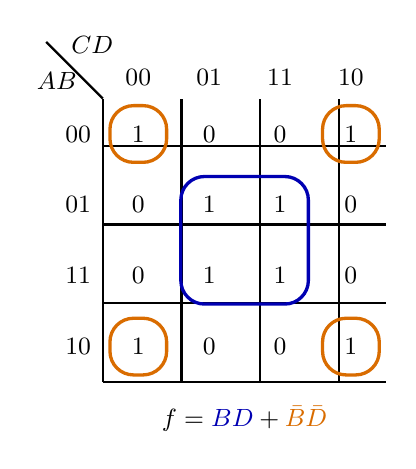
\begin{tikzpicture}[x=9mm, y=9mm, every node/.style={font=\small}]
  \draw[thick] (0,0) grid (4,4);
  \draw[thick] (0,4) -- (-0.8,4.8);
  \node at (-0.65,4.25) {$AB$};
  \node at (-0.15,4.75) {$CD$};
  \foreach \v [count=\i from 0] in {00, 01, 11, 10} {
    \node at (\i + 0.5, 4.3) {$\v$};
    \node at (-0.35, 3.5 - \i) {$\v$};
  }
  \foreach \row [count=\r] in {{1,0,0,1}, {0,1,1,0}, {0,1,1,0}, {1,0,0,1}}
    \foreach \v [count=\c] in \row
      \node at (\c - 0.5, 4.5 - \r) {$\v$};

  \draw[blue!70!black, very thick, rounded corners=3mm] (1.1,1.1) rectangle (2.9,2.9);
  \foreach \x/\y in {0/0, 3/0, 0/3, 3/3}
    \draw[orange!85!black, very thick, rounded corners=3mm] (\x + 0.1,\y + 0.1) rectangle (\x + 0.9,\y + 0.9);
  \node[below] at (2,-0.2) {$f = {\color{blue!70!black} BD} + {\color{orange!85!black} \bar{B}\bar{D}}$};
\end{tikzpicture}
